\documentclass[10pt,conference]{IEEEtran}

\usepackage{url,graphicx,subfigure,algcompatible,comment,amsmath,units,epsfig,threeparttable,multirow,colortbl,booktabs,setspace,textcomp}


\usepackage[ruled]{algorithm2e}

\title{An Agile Migration Framework for Analog Layout Design}
\author{
\IEEEauthorblockN{Po-Cheng Pan\IEEEauthorrefmark{1}, Prof. Hung-Ming Chen\IEEEauthorrefmark{1}\\}
\IEEEauthorblockA{\IEEEauthorrefmark{1}Institute of Electronics and SoC Center, National Chiao Tung University, Hsinchu, Taiwan\\}
\IEEEauthorblockA{Email: benbean.ee96g@g2.nctu.edu.tw; hmchen@mail.nctu.edu.tw}

  %\thanks{
  %{\scriptsize
  %  This work was partially supported by the National Science Council of Taiwan ROC under grant No. NSC 102-2220-E-009-024
    

  %  \noindent
  %  978-1-4799-1071-7/13/\$31.00 \copyright2013 IEEE }
  %}
}

\begin{document}

\maketitle

\begin{abstract}
  Layout generation in the late analog CMOS design is challenging by its increasing layout constraints and performance requirements. However, iterative refinement on manual design damages the productivity of analog layout. Therefore, it is more efficient to enroll the know-how from existing design instead of generating a new one. To contend with time-consuming analog layout for more possibilities, this software aims to demonstrate a fast layout prototyping framework for migration purpose into real layout design.

  In our framework, a reference analog layout design is given to generate potential layout candidates at the objective technology. The demonstration includes the original layout, the extracted topology with placement and routing, the generated layout figures, the dumped layout results and the simulated results. This procedure of migration provides a convincing exhibition of our migration framework.
\end{abstract}

%! ROOT TEX = UnivBooth_DATE15.tex

\section{Background and Related Work}

  The application of analog layout generation is widely developed in academia and industry. Commercial tools like Cadence Virtuoso ADE, Synopsys Laker have provided template-based schematic-driven analog layout generator. However, the generated layout mostly keeps the original topology. Our software integrates mechanisms from \cite{ALP_YPWeng_iccad2011,Chin_DMR_ICCAD2013,PAGE_DATE2013}. The device sizes of targeting technology is generated from \cite{PAGE_DATE2013}. In \cite{ALP_YPWeng_iccad2011}, it provides multiple placement results withholding analog layout constraints. For routing generation, \cite{Chin_DMR_ICCAD2013} preserves the behavior of routing from the reference layout and fast generates routing on the targeting layout.

   

\section{Flow of Our Framework}
  \begin{figure}[ht]
    \centering
    \centerline{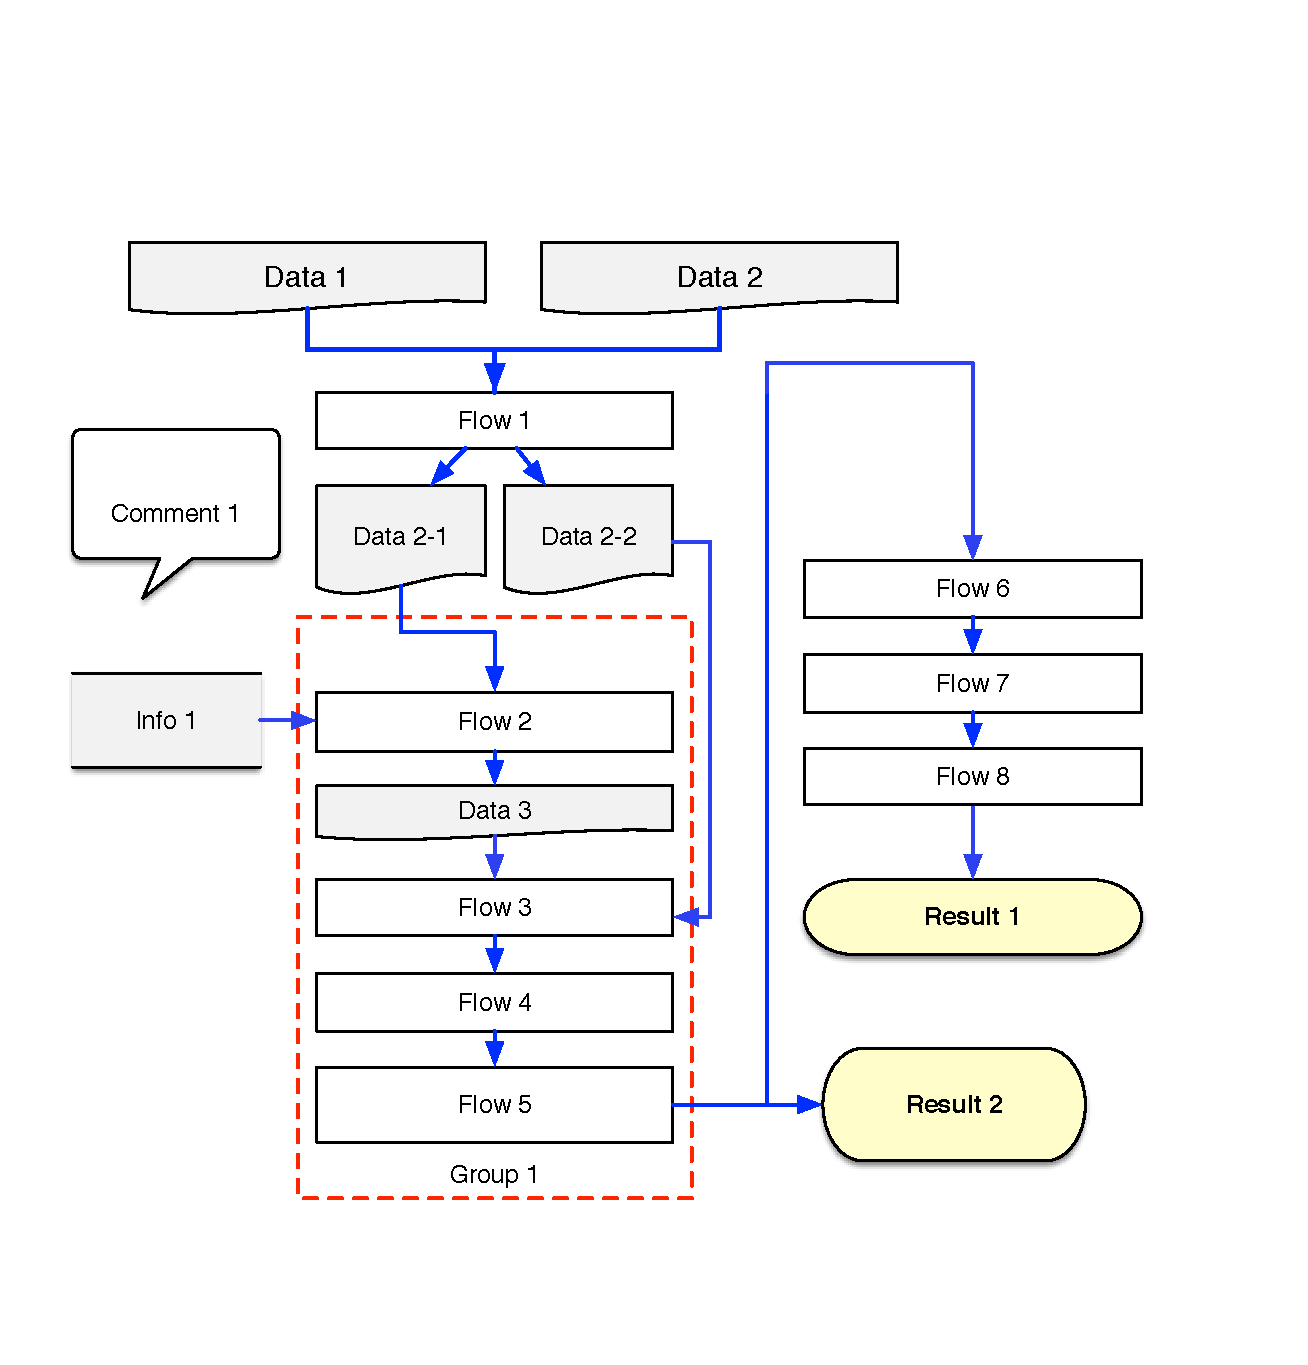
\epsfig{file=Fig/proto_flow.eps,height=7cm}}
    \caption{Overall flow of the proposed layout migration framework.} 
    \centering{\label{fig:Flow}}
  \end{figure}


  In order to provide fast prototyping for layout migration, this software extracted the reference layout with placement and routing respectively. The migrated layout is generated according to the extracted information. and then it dumps into real design after physical verification for performance simulation. Fig.~\ref{fig:Flow} shows the overall flow diagram of our methodology.
  The flow is mainly separated into three stages: 
  \begin{enumerate}
    \item {\bf Extraction and Preservation}: A layout extraction and preservation technique \cite{Chin_DMR_ICCAD2013} can not only be applied to generalized layout, but also hierarchical design.
    \item {\bf Prototyping}: The preserved topology of original layout can be generated into multiple layout candidates with placement and routing. 
    \item {\bf Wire optimization}: A detailed routing refinement is applied automatically to route the unrouted nets for final verification and simulation.
  \end{enumerate}

  In the end, a set of layouts with refinement is obtained, which provides designers a quick look of possible solutions that can be used. The layout results are automatically dumped into industrial layouts for demonstration and simulation. 


\section{Program Setting and Results}
  
  Our Software is developed with g++ 4.1.2 for methodology, Synopsys $\text{PyCell Studio}^{\text{TM} }$ 4.7.1 for layout realization and Qt 4.8.4 for GUI demonstration. We also display the layout with the reference one and the generated layout via $\text{Cadence}^{\text{\textregistered}}$ $\text{Virtuoso}^{\text{\textregistered}}$ 6.1.5. The migration of a variable-gain amplifier (VGA), a folded-cascode operational amplifier (OpAmp) and low dropout regulator (LDO) will be demonstrated step-by-step as applications to show the feasibility of our Software. 
  %for migration and hierarchical prototypes generation. The numerical results of routing and performance are listed in Table~\ref{table:MigrationPerf}. Comparing with manual layout (ML), the preserved prototyping layout (PPL) earns better design time with qualified performance. 
  %Moreover, PPL also rewords better routing completness than non-preserved automatic layout (NAL). 
  %These results demonstrate that the proposed framework effectively contributes the reusability of analog layout and efficiently boosts the productivity with qualified performance. 

  %Our contributions not only favor advanced analog IC industries, but also raise a practical application for constrained Delaunay triangulation. We tend to submit this work to Design Automation and Testing in Europe, Design Automation Conference, International Conference on Computer-Aided Design in the near future.



\bibliographystyle{IEEEtran}
\bibliography{IEEEfull,IEEEabrv,IEEEexample,reference}

\end{document}